%%%%%%%%%%%%%%%%%%%%%%%%%%%%%%%%%%%%%%%%%%%%%%%%%%%%%%%%%%
\frame {\frametitle{Spark Components}
%%%%%%%%%%%%%%%%%%%%%%%%%%%%%%%%%%%%%%%%%%%%%%%%%%%%%%%%%%
\begin{figure}[h]
  \centering
  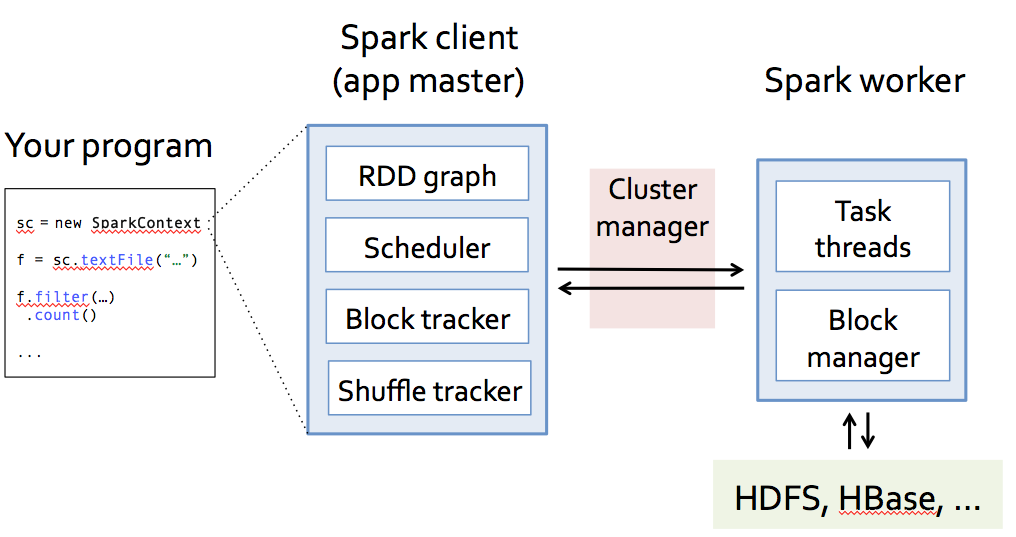
\includegraphics[scale=0.33]{./Figures/spark_components}
  \label{fig:spark_components}
\end{figure}
}

%%%%%%%%%%%%%%%%%%%%%%%%%%%%%%%%%%%%%%%%%%%%%%%%%%%%%%%%%%
\frame {\frametitle{Lifetime of a Job in Spark}
%%%%%%%%%%%%%%%%%%%%%%%%%%%%%%%%%%%%%%%%%%%%%%%%%%%%%%%%%%

\begin{columns}[t, onlytextwidth]
	\begin{column}[T]{.2\textwidth}
		\begin{center}
			{ \tiny \bf RDD Objects}
		\end{center}
		\begin{figure}[h]
			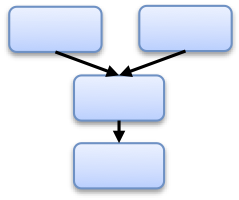
\includegraphics[scale=0.5]{./Figures/RDD_objects}
		\end{figure}

		\begin{colorblock}{blue}{lightblue}{ }
			{\tiny \texttt{
				rdd1.join(rdd2)\\
				\hspace{12pt} .groupBy(...)\\
				\hspace{12pt} .filter(...)\\
				}
			}
		\end{colorblock}

		\vspace{10pt}

		\begin{colorblock}{blue}{lightblue}{ }
			{\tiny \bf Build the operator DAG}
		\end{colorblock}
	\end{column}

	\begin{column}[T]{.2\textwidth}
		\begin{center}
			{ \tiny \bf DAG Scheduler}
		\end{center}			
		\begin{figure}[h]
			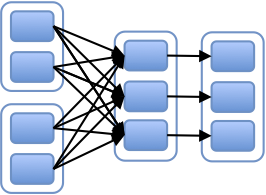
\includegraphics[scale=0.5]{./Figures/DAG_scheduler}
		\end{figure}

		\vspace{10pt}

		\begin{colorblock}{blue}{lightblue}{ }
			{\tiny \bf Split the DAG into \emph{stages} of \emph{tasks}}
		\end{colorblock}

		\vspace{10pt}

		\begin{colorblock}{blue}{lightblue}{ }
			{\tiny \bf Submit each stage and its tasks as ready}
		\end{colorblock}			
	\end{column}

	\begin{column}[T]{.2\textwidth}
		\begin{center}
			{ \tiny \bf Task Scheduler}
		\end{center}			

		\vspace{-20pt}

		\begin{figure}[h]
			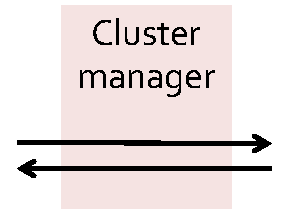
\includegraphics[scale=0.5]{./Figures/Task_scheduler}
		\end{figure}

		\vspace{10pt}

		\begin{colorblock}{blue}{lightblue}{ }
			{\tiny \bf Launch tasks via Master}
		\end{colorblock}

		\vspace{10pt}

		\begin{colorblock}{blue}{lightblue}{ }
			{\tiny \bf Retry failed and straggler tasks}
		\end{colorblock}			
	\end{column}

	\begin{column}[T]{.2\textwidth}
		\begin{center}
			{ \tiny \bf Worker}
		\end{center}			
		\begin{figure}[h]
			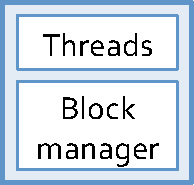
\includegraphics[scale=0.5]{./Figures/Worker}
		\end{figure}
		\vspace{10pt}

		\begin{colorblock}{blue}{lightblue}{ }
			{\tiny \bf Execute tasks}
		\end{colorblock}

		\vspace{10pt}

		\begin{colorblock}{blue}{lightblue}{ }
			{\tiny \bf Store and serve blocks}
		\end{colorblock}			
	\end{column}
\end{columns}
}

%%%%%%%%%%%%%%%%%%%%%%%%%%%%%%%%%%%%%%%%%%%%%%%%%%%%%%%%%%
\frame {\frametitle{What is an RDD}
%%%%%%%%%%%%%%%%%%%%%%%%%%%%%%%%%%%%%%%%%%%%%%%%%%%%%%%%%%
\begin{itemize}
	\item {\bf RDD are partitioned, locality aware, distributed collections}

	\vspace{20pt}

	\item {\bf RDD are data structures that:}
	\begin{itemize}
		\item Either point to a direct data source (e.g. HDFS)
		\item Apply some transformations to its parent RDD(s) to generate new data elements
	\end{itemize}

	\vspace{20pt}

	\item {\bf Computations on RDDs}
	\begin{itemize}
	 	\item Represented by \emph{lazily evaluated} lineage \emph{DAGs} composed by chained RDDs
	 \end{itemize} 
\end{itemize}
}

%%%%%%%%%%%%%%%%%%%%%%%%%%%%%%%%%%%%%%%%%%%%%%%%%%%%%%%%%%
\frame {\frametitle{RDD Abstraction}
%%%%%%%%%%%%%%%%%%%%%%%%%%%%%%%%%%%%%%%%%%%%%%%%%%%%%%%%%%
\begin{itemize}
	\item {\bf Overall objective}
	\begin{itemize}
		\item Support a wide array of operators (more than just \texttt{Map} and \texttt{Reduce})
		\item Allow arbitrary composition of such operators
	\end{itemize}

	\vspace{20pt}

	\item {\bf Simplify scheduling}
	\begin{itemize}
		\item Avoid to modify the scheduler for each operator
	\end{itemize}

	\vspace{20pt}

	\item[$\to$] The question is: \emph{How to capture dependencies in a general way?}
\end{itemize}
}

%%%%%%%%%%%%%%%%%%%%%%%%%%%%%%%%%%%%%%%%%%%%%%%%%%%%%%%%%%
\frame {\frametitle{RDD Interfaces}
%%%%%%%%%%%%%%%%%%%%%%%%%%%%%%%%%%%%%%%%%%%%%%%%%%%%%%%%%%
\begin{itemize}
	\item {\bf Set of partitions (``splits'')}
	\begin{itemize}
		\item Much like in Hadoop MapReduce, each RDD is associated to (input) partitions
	\end{itemize}

	\item {\bf List of dependencies on parent RDDs}
	\begin{itemize}
		\item This is completely new w.r.t. Hadoop MapReduce
	\end{itemize}

	\item {\bf Function to compute a partition given parents}
	\begin{itemize}
		\item This is actually the ``user-defined code'' we referred to when discussing about the \texttt{Mapper} and \texttt{Reducer} classes in Hadoop
	\end{itemize}

	\item {\bf Optional preferred locations}
	\begin{itemize}
		\item This is to enforce data locality
	\end{itemize}

	\item {\bf Optional partitioning info (Partitioner)}
	\begin{itemize}
		\item This really helps in some ``advanced'' scenarios in which you want to pay attention to the behavior of the shuffle mechanism
	\end{itemize}
\end{itemize}
}

%%%%%%%%%%%%%%%%%%%%%%%%%%%%%%%%%%%%%%%%%%%%%%%%%%%%%%%%%%
\frame {\frametitle{Hadoop RDD}
%%%%%%%%%%%%%%%%%%%%%%%%%%%%%%%%%%%%%%%%%%%%%%%%%%%%%%%%%%
\begin{itemize}
	\item Slide 15 MZ
\end{itemize}

}

%%%%%%%%%%%%%%%%%%%%%%%%%%%%%%%%%%%%%%%%%%%%%%%%%%%%%%%%%%
\frame {\frametitle{Filtered RDD}
%%%%%%%%%%%%%%%%%%%%%%%%%%%%%%%%%%%%%%%%%%%%%%%%%%%%%%%%%%
\begin{itemize}
	\item Slide 16 MZ
\end{itemize}

}

%%%%%%%%%%%%%%%%%%%%%%%%%%%%%%%%%%%%%%%%%%%%%%%%%%%%%%%%%%
\frame {\frametitle{Joined RDD}
%%%%%%%%%%%%%%%%%%%%%%%%%%%%%%%%%%%%%%%%%%%%%%%%%%%%%%%%%%
\begin{itemize}
	\item Slide 17 MZ
\end{itemize}
}

%%%%%%%%%%%%%%%%%%%%%%%%%%%%%%%%%%%%%%%%%%%%%%%%%%%%%%%%%%
\frame {\frametitle{Dependency Types}
%%%%%%%%%%%%%%%%%%%%%%%%%%%%%%%%%%%%%%%%%%%%%%%%%%%%%%%%%%
\begin{itemize}
	\item Slide 18 MZ
\end{itemize}

}

%%%%%%%%%%%%%%%%%%%%%%%%%%%%%%%%%%%%%%%%%%%%%%%%%%%%%%%%%%
\frame {\frametitle{RDD Code Snippet}
%%%%%%%%%%%%%%%%%%%%%%%%%%%%%%%%%%%%%%%%%%%%%%%%%%%%%%%%%%
\begin{itemize}
	\item Slide 11 Taro Saito
\end{itemize}
}

%%%%%%%%%%%%%%%%%%%%%%%%%%%%%%%%%%%%%%%%%%%%%%%%%%%%%%%%%%
\frame {\frametitle{RDD Map operation Snippet}
%%%%%%%%%%%%%%%%%%%%%%%%%%%%%%%%%%%%%%%%%%%%%%%%%%%%%%%%%%
\begin{itemize}
	\item Slide 12 Taro Saito
\end{itemize}

}

%%%%%%%%%%%%%%%%%%%%%%%%%%%%%%%%%%%%%%%%%%%%%%%%%%%%%%%%%%
\frame {\frametitle{RDD Iterator Code Snipped}
%%%%%%%%%%%%%%%%%%%%%%%%%%%%%%%%%%%%%%%%%%%%%%%%%%%%%%%%%%
\begin{itemize}
	\item Slide 13 Taro Saito
\end{itemize}

}

%%%%%%%%%%%%%%%%%%%%%%%%%%%%%%%%%%%%%%%%%%%%%%%%%%%%%%%%%%
\frame {\frametitle{Making RDD from local collections}
%%%%%%%%%%%%%%%%%%%%%%%%%%%%%%%%%%%%%%%%%%%%%%%%%%%%%%%%%%
\begin{itemize}
	\item Slide 29 Taro Saito
\end{itemize}
}

%%%%%%%%%%%%%%%%%%%%%%%%%%%%%%%%%%%%%%%%%%%%%%%%%%%%%%%%%%
\frame {\frametitle{Hadoop RDD Code Snippet}
%%%%%%%%%%%%%%%%%%%%%%%%%%%%%%%%%%%%%%%%%%%%%%%%%%%%%%%%%%
\begin{itemize}
	\item Slide 30 Taro Saito
\end{itemize}
}

%%%%%%%%%%%%%%%%%%%%%%%%%%%%%%%%%%%%%%%%%%%%%%%%%%%%%%%%%%
\begin{frame}[fragile]
\frametitle{A Very Simple Job Example}
%%%%%%%%%%%%%%%%%%%%%%%%%%%%%%%%%%%%%%%%%%%%%%%%%%%%%%%%%%


\begin{lstlisting}
val sc = new SparkContext("spark://...", "MyJob", home, jars) 

val file = sc.textFile("hdfs://...") // This is an RDD

val errors = file.filter(_.contains("ERROR")) // This is an RDD

errors.cache()

errors.count() // This is an action
\end{lstlisting}

\end{frame}


%%%%%%%%%%%%%%%%%%%%%%%%%%%%%%%%%%%%%%%%%%%%%%%%%%%%%%%%%%
\frame {\frametitle{The RDD graph: dataset vs. partition views}
%%%%%%%%%%%%%%%%%%%%%%%%%%%%%%%%%%%%%%%%%%%%%%%%%%%%%%%%%%
% missing: what is an rdd? difference between RDD and partition?

\begin{columns}[c]
	\column{.5\textwidth}
		
			\begin{figure}[h]
			  \centering
			  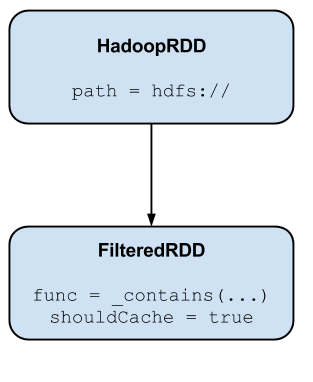
\includegraphics[scale=0.25]{./Figures/spark_rdd}
			  \label{fig:spark_components}
			\end{figure}
	
	\column{.5\textwidth}
		
			\begin{figure}[h]
			  \centering
			  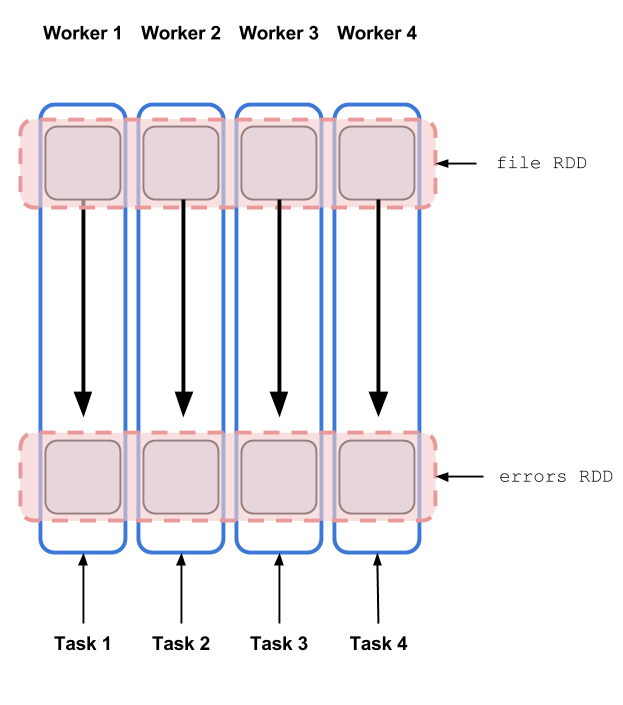
\includegraphics[scale=0.25]{./Figures/spark_partition}
			  \label{fig:spark_components}
			\end{figure}

\end{columns}
}

% %%%%%%%%%%%%%%%%%%%%%%%%%%%%%%%%%%%%%%%%%%%%%%%%%%%%%%%%%%
% \frame {\frametitle{Data Locality}
% %%%%%%%%%%%%%%%%%%%%%%%%%%%%%%%%%%%%%%%%%%%%%%%%%%%%%%%%%%
% \begin{itemize}
% 	\item First run: data not in cache, so use HadoopRDD's locality prefs (from HDFS)
% 	\item Second run: FilteredRDD is in cache, so use its locations
% 	\item If something falls out of cache, go back to HDFS
% \end{itemize}
% }
